%-----------------------------------------------------------------------------------------------
\makeatletter
\immediate\write18{datelog > \jobname.info} % site script for $(date '+%Y-%m-%d %Hh%Mm%Ss')
\makeatother
%-----------------------------------------------------------------------------------------------
%-----------------------------------------------------------------------------------------------
\usetheme{Copenhagen}
\usepackage{beamercolorthemeUTF2}
\usefonttheme{serif}
%-----------------------------------------------------------------------------------------------
\usepackage[utf8]{inputenc}
\usepackage[greek,french,english,brazil]{babel} % last becomes the active one
\usepackage{pslatex}
\usepackage{amssymb,amsmath}
\usepackage{soul}
\usepackage[squaren,Gray,cdot]{SIunits}
\usepackage[nice]{nicefrac}
\usepackage{tikz}
\usepackage{amscd}
\usepackage{stmaryrd}
\usepackage{scalerel}
\usepackage{xspace}
%-----------------------------------------------------------------------------------------------


%-----------------------------------------------------------------------------------------------
%-----------------------------------------------------------------------------------------------
% Mathematical
%-----------------------------------------------------------------------------------------------
\newcommand{\vet}[1]{\underline{{#1}}}
\newcommand{\mat}[1]{\underline{\underline{{#1}}}}
\newcommand{\cub}[1]{\underline{\underline{\underline{{#1}}}}}
\newcommand{\eqdef}{{\ensuremath\stackrel{\text{\tiny def}}{=}}}
%-----------------------------------------------------------------------------------------------
% Linguistic
%-----------------------------------------------------------------------------------------------
\newcommand{\GRtxt}[1]{\begin{otherlanguage}{greek}{{#1}}\end{otherlanguage}}
\newcommand{\FRtxt}[1]{\begin{otherlanguage}{french}{{#1}}\end{otherlanguage}}
%-----------------------------------------------------------------------------------------------
% Presentation
%-----------------------------------------------------------------------------------------------
\newcommand{\BkgImgH}[1]{% Places an image centered on the slide background filling the height
    \usebackgroundtemplate{\parbox{\paperwidth}{%
        \vspace*{1sp}\centering\includegraphics[height=\paperheight]{{#1}}
}}}
\newcommand{\BkgImgW}[1]{% Places an image centered on the slide background filling the width
    \usebackgroundtemplate{\parbox{\paperwidth}{%
        \vspace*{1sp}\centering\includegraphics[width=\paperwidth]{{#1}}
}}}
\newcommand{\ArtEndH}[3]{% Transitions to plain image (last) slide: #1:prefix #2,#3:extensions
    \BkgImgH{root/../art/#1.#2}
    \frame<handout:0>[plain]{%
        \transdissolve\vspace*{72mm}\color{white}\scriptsize\bf\input{root/../art/#1.#3}}
    \usebackgroundtemplate{\mbox{~}}
}
\newcommand{\ArtEndW}[3]{% Transitions to plain image (last) slide: #1:prefix #2,#3:extensions
    \BkgImgW{root/../art/#1.#2}
    \frame<handout:0>[plain]{%
        \transdissolve\vspace*{72mm}\color{white}\scriptsize\bf\input{root/../art/#1.#3}}
    \usebackgroundtemplate{\mbox{~}}
}
\newcommand{\ImgColW}[3]{% Inserts a full-width image in a column
    \includegraphics[width=\columnwidth]{root/../art/#1.#2}\\[-0.5\baselineskip]
    \parbox{\columnwidth}{\tiny\hfill\scalebox{0.85}{\input{root/../art/#1.#3}}}
}
\newcommand{\txtpic}[1]{%
    \fcolorbox{lightgray}{white!90!black}{{#1}} 
}
%-----------------------------------------------------------------------------------------------


%-----------------------------------------------------------------------------------------------
\title{A.03.04 -- Modelos de Propriedades Energéticas}
\subtitle{(Sistemas Fechados)}
\author{Prof.~C.~Naaktgeboren, PhD}
\date{{\scriptsize\tt%
    
\includegraphics[height=6.0mm]{root/00-res/cc/by-nc-nd-88x31.pdf}\\[\smallskipamount]
    https://github.com/CNThermSci/ApplThermSci\\
    Compiled on \input{\jobname.info}
}}
%-----------------------------------------------------------------------------------------------
\begin{document}
%-----------------------------------------------------------------------------------------------
\logo{%
    \parbox{158mm}{% There's a 1mm gap on each side of the 160mm x 90mm slide logo line
        \mode<beamer>{
            
\includegraphics[height=6.0mm]{root/00-res/UTFPR/UTFPR-logo-D.pdf}\hfill%
            
\includegraphics[height=9.0mm]{root/00-res/logo/CNThermSci-logo-A.pdf}%
        }
        \mode<handout>{
            
\includegraphics[height=6.0mm]{root/00-res/UTFPR/UTFPR-logo-W.pdf}\hfill%
            
\includegraphics[height=9.0mm]{root/00-res/logo/CNThermSci-logo-W.pdf}%
        }
    }
} % The (delineated, alpha), or washed-out logos
%-----------------------------------------------------------------------------------------------
\frame{\titlepage}
%-----------------------------------------------------------------------------------------------

%-----------------------------------------------------------------------------------------------
\frame{\tableofcontents}
%-----------------------------------------------------------------------------------------------

%-----------------------------------------------------------------------------------------------
\section{Modelos de Propriedades Energéticas}
%-----------------------------------------------------------------------------------------------

%-----------------------------------------------------------------------------------------------
\subsection{Energia Interna e Entalpia}
%-----------------------------------------------------------------------------------------------

    % !j 96 -i8
    %-------------------------------------------------------------------------------------------
    \begin{frame}{Energia Interna -- Relação com Temperatura}\vspace*{-2em}
        \begin{columns}
        \column{0.55\textwidth}
            O sistema fechado de massa \alert{$m$}, ilustrado:\\[\smallskipamount]
            \begin{itemize}
                \item<1-> Recebe uma diferencial de calor a  volume  constante,  \alert{$(\delta
                    q)_V$};
                \item<2-> \alert{$m$} e \alert{$V$}  constantes  implicam  em  \alert{$v  \equiv
                    V/m$} constante, tal que \alert{$(\delta q)_V = (\delta q)_v$};
                \item<3-> A temperatura experimenta uma variação de \alert{$(dT)_v$}.
            \end{itemize}
        \column{0.45\textwidth}
            \begin{figure}
                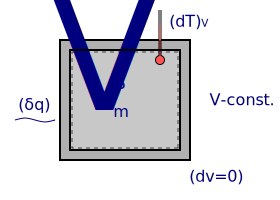
\includegraphics[width=5.0cm]{fig/A0304-pt-ConstVHeating.pdf}
            \end{figure}
        \end{columns}
    \end{frame}
    %-------------------------------------------------------------------------------------------

    % !j 96 -i8
    %-------------------------------------------------------------------------------------------
    \begin{frame}{Energia Interna -- Relação com Temperatura (Cont.)}\vspace*{-2em}
        \begin{columns}
        \column{0.55\textwidth}
            O balanço de energia na forma diferencial do sistema fica:
            \begin{align}
                \uncover<2->{\delta e_{ent} - \delta e_{sai} & = de_{sist}\quad}
                \uncover<3->{\rightharpoondown\nonumber\\(\delta q)_v & = du.\nonumber}
            \end{align}
            \uncover<4->{%
                Assim, \alert{o calor transferido a volume constante a um sistema fechado é a
                variação de sua energia interna}!
            }
        \column{0.45\textwidth}
            \begin{figure}
                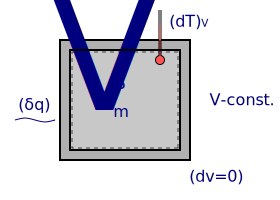
\includegraphics[width=5.0cm]{fig/A0304-pt-ConstVHeating.pdf}
            \end{figure}
        \end{columns}
    \end{frame}
    %-------------------------------------------------------------------------------------------

    % !j 96 -i8
    %-------------------------------------------------------------------------------------------
    \begin{frame}{Energia Interna -- Relação com Temperatura (Cont.)}\vspace*{-2em}
        \begin{columns}
        \column{0.55\textwidth}
            Define-se o \alert{calor específico a volume constante} da substância do sistema,
            $c_v$, como
            \begin{align}
                \uncover<1->{\alert{c_v} & \alert{\equiv}}
                \uncover<1->{\alert{\left(\frac{\partial u}{\partial T}\right)_v},\nonumber}
            \end{align}
            \uncover<1->{%
                \noindent uma \alert{propriedade} termodinâmica intensiva.
            }\\[\medskipamount]
            \uncover<2->{%
                Ainda, $C_v = (\partial U /  \partial  T)_v  =  m\,c_v$  é  a  \alert{capacidade
                térmical a volume constante} do sistema.
            }
        \column{0.45\textwidth}
            \begin{figure}
                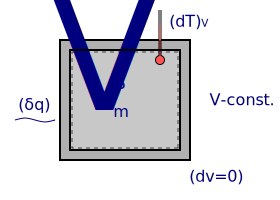
\includegraphics[width=5.0cm]{fig/A0304-pt-ConstVHeating.pdf}
            \end{figure}
        \end{columns}
    \end{frame}
    %-------------------------------------------------------------------------------------------

    % !j 96 -i8
    %-------------------------------------------------------------------------------------------
    \begin{frame}{Entalpia -- Relação com Temperatura}\vspace*{-2em}
        \begin{columns}
        \column{0.55\textwidth}
            O sistema fechado de massa \alert{$m$}, ilustrado:\\[\smallskipamount]
            \begin{itemize}
                \item<1-> Recebe uma diferencial de calor a pressão  constante,  \alert{$(\delta
                    q)_P$};
                \item<2->  Realiza  uma   diferencial   de   trabalho   a   pressão   constante,
                    \alert{$(\delta w)_P = P\,dv$};
                \item<3->  A  temperatura  experimenta   uma   variação   de   \alert{$(dT)_P$},
                    possivelmente diferente de $(dT)_v$.
            \end{itemize}
        \column{0.45\textwidth}
            \begin{figure}
                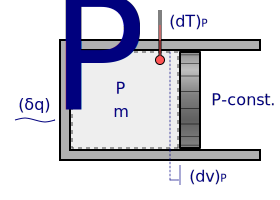
\includegraphics[width=5.0cm]{fig/A0304-pt-ConstPHeating.pdf}
            \end{figure}
        \end{columns}
    \end{frame}
    %-------------------------------------------------------------------------------------------

    % !j 96 -i8
    %-------------------------------------------------------------------------------------------
    \begin{frame}{Entalpia -- Relação com Temperatura (Cont.)}\vspace*{-2em}
        \begin{columns}
        \column{0.55\textwidth}
            O balanço de energia na forma diferencial do sistema fica:
            \begin{align}
                \uncover<2->{\delta e_{ent} - \delta e_{sai} & = de_{sist}\quad}
                \uncover<3->{\rightharpoondown\nonumber\\}
                \uncover<3->{(\delta q)_P - (\delta w)_P & = du\quad}
                \uncover<4->{\rightharpoondown\nonumber\\}
                \uncover<4->{\alert{(\delta q)_P} & = du + P\,dv \alert{= d(u + Pv)}.\nonumber}
            \end{align}
            \uncover<5->{%
                A quantidade \alert{$(u + Pv)$} aparece frequentemente  o  suficiente  para  ser
                definida como uma nova propriedade.
            }
        \column{0.45\textwidth}
            \begin{figure}
                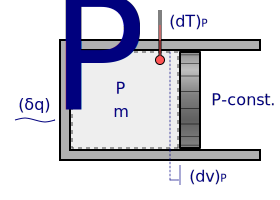
\includegraphics[width=5.0cm]{fig/A0304-pt-ConstPHeating.pdf}
            \end{figure}
        \end{columns}
    \end{frame}
    %-------------------------------------------------------------------------------------------

    % !j 96 -i8
    %-------------------------------------------------------------------------------------------
    \begin{frame}{Entalpia -- Relação com Temperatura (Cont.)}\vspace*{-2em}
        \begin{columns}
        \column{0.55\textwidth}
            Assim,
            \begin{align}
                \uncover<1->{%
                    \alert{H} & \alert{\equiv U + PV} && [\kilo\joule]\mbox{, e}\nonumber\\}
                \uncover<2->{%
                    \alert{h} & \alert{\equiv u + Pv} && [\kilo\joule\per\kilogram],\nonumber}
            \end{align}
            \uncover<3->{%
                \noindent   são   a   \alert{entalpia}   e   a   \alert{entalpia    específica},
                respectivamente: novas propriedades termodinâmicas.
            }
        \column{0.45\textwidth}
            \begin{figure}
                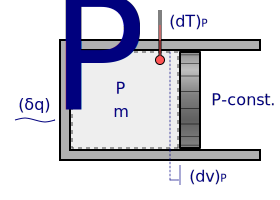
\includegraphics[width=5.0cm]{fig/A0304-pt-ConstPHeating.pdf}
            \end{figure}
        \end{columns}
    \end{frame}
    %-------------------------------------------------------------------------------------------

    % !j 96 -i8
    %-------------------------------------------------------------------------------------------
    \begin{frame}{Entalpia -- Relação com Temperatura (Cont.)}\vspace*{-2em}
        \begin{columns}
        \column{0.55\textwidth}
            \uncover<1->{%
                O termo origina do  verbo  grego  \alert{``\GRtxt{enj'alpw}''},  que  significa:
                \alert{``(eu) aqueço''}, conforme a própria ilustração.
            }\\[\medskipamount]
            \uncover<2->{%
                Da expressão \alert{$(\delta q)_P = dh$}, tem-se que \alert{o calor  transferido
                a pressão constante a um sistema fechado é a variação de sua entalpia}!
            }
        \column{0.45\textwidth}
            \begin{figure}
                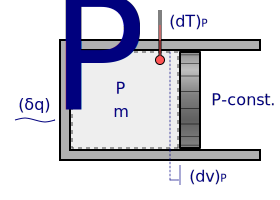
\includegraphics[width=5.0cm]{fig/A0304-pt-ConstPHeating.pdf}
            \end{figure}
        \end{columns}
    \end{frame}
    %-------------------------------------------------------------------------------------------

    % !j 96 -i8
    %-------------------------------------------------------------------------------------------
    \begin{frame}{Entalpia -- Relação com Temperatura (Cont.)}\vspace*{-2em}
        \begin{columns}
        \column{0.55\textwidth}
            Define-se o \alert{calor específico a pressão constante} da substância  do  sistema,
            $c_P$, como
            \begin{align}
                \uncover<1->{\alert{c_P} & \alert{\equiv}}
                \uncover<1->{\alert{\left(\frac{\partial h}{\partial T}\right)_P},\nonumber}
            \end{align}
            \uncover<1->{%
                \noindent uma \alert{propriedade} termodinâmica intensiva.
            }\\[\medskipamount]
            \uncover<2->{%
                Ainda, $C_P = (\partial H /  \partial  T)_P  =  m\,c_P$  é  a  \alert{capacidade
                térmical a pressão constante} do sistema.
            }
        \column{0.45\textwidth}
            \begin{figure}
                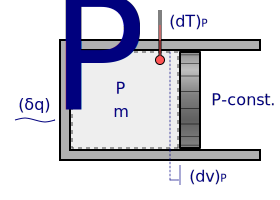
\includegraphics[width=5.0cm]{fig/A0304-pt-ConstPHeating.pdf}
            \end{figure}
        \end{columns}
    \end{frame}
    %-------------------------------------------------------------------------------------------

%-----------------------------------------------------------------------------------------------
\subsection{$U$ e $H$ em Modelos de Substâncias}
%-----------------------------------------------------------------------------------------------

    % !j 96 -i8
    %-------------------------------------------------------------------------------------------
    \begin{frame}{Gás Ideal --- Substância com $Pv = RT$}\vspace*{-2em}
        \begin{columns}
        \column{0.50\textwidth}
            Experimentos mostraram que \alert{$u\!:\!u(T)$}, assim,
            \begin{align}
                \uncover<2->{\delta q - \delta w & = du}
                \uncover<3->{\quad\rightharpoondown\nonumber\\}
                \uncover<3->{(\delta q)_T - (\delta w)_T & = (du)_T = 0}
                \uncover<4->{\quad\rightharpoondown\nonumber\\}
                \uncover<4->{\alert{(\delta q)_T} & \alert{= (\delta w)_T}.\nonumber}
            \end{align}
            \uncover<5->{A definição de $c_v$ simplifica para}\\[-2.00ex]
            \begin{align}
                \uncover<5->{c_v(T) & = \frac{du}{dT}}
                \uncover<6->{\quad\rightharpoondown\nonumber\\}
                \uncover<6->{\alert{u(T)} & \alert{= \int c_v(T)\,dT}.\nonumber}
            \end{align}
        \column{0.50\textwidth}
            \uncover<7->{Ainda,}
            \begin{align}
                \uncover<8->{h & \equiv u + Pv}
                \uncover<9->{\quad\rightharpoondown\nonumber\\}
                \uncover<9->{h & = u + RT,\nonumber}
            \end{align}
            \uncover<10->{\noindent fazendo com que \alert{$h\!:\!h(T)$}, e ainda}
            \begin{align}
                \uncover<10->{c_P(T) & = \frac{dh}{dT} = \frac{du + R\,dT}{dT}}
                \uncover<11->{\quad\rightharpoondown\nonumber\\}
                \uncover<11->{\alert{h(T)} & \alert{= \int c_P(T)\,dT}}
                \uncover<12->{\quad\mbox{and}\nonumber\\}
                \uncover<12->{\alert{c_P(T)} & \alert{= c_v(T) + R}.\nonumber}
            \end{align}
        \end{columns}
    \end{frame}
    %-------------------------------------------------------------------------------------------

    % !j 96 -i8
    %-------------------------------------------------------------------------------------------
    \begin{frame}{Gás Ideal --- Calores Específicos}\vspace*{-2em}
        \begin{align}
            \uncover<1->{\alert{c_P(T)} & \alert{= c_v(T) + R} && (\kilo\joule\per\kilogram)}
            \uncover<2->{\quad\rightharpoondown\nonumber\\[\smallskipamount]}
            \uncover<2->{\alert{\bar{c}_P(T)} & \alert{= \bar{c}_v(T) + \bar{R}} && (\kilo\joule\per\kilo\mole)}
            \uncover<3->{\nonumber\\[\smallskipamount]}
            \uncover<3->{\alert{\gamma(T)} & \alert{\equiv \frac{c_P(T)}{c_v(T)}}}
            \uncover<3->{= 1 + \frac{R}{c_v(T)} && (\mbox{---})}
            \uncover<4->{\nonumber\\[\smallskipamount]}
            \uncover<4->{\bar{c}_{P,monatom.} &= \nicefrac{5}{2}\bar{R}\nonumber\\[\smallskipamount]}
            \uncover<5->{\bar{c}_{P,di-atom.} &= \nicefrac{7}{2}\bar{R}\nonumber\\[\smallskipamount]}
            \uncover<6->{\gamma_{He} &= \nicefrac{5}{3} \approx 1,667\nonumber\\[\smallskipamount]}
            \uncover<7->{\gamma_{ar}(\unit{300}{\kelvin}) &\approx \nicefrac{7}{5} = 1,4.\nonumber}
        \end{align}
    \end{frame}
    %-------------------------------------------------------------------------------------------

    % !j 96 -i8
    %-------------------------------------------------------------------------------------------
    \begin{frame}{Gás Ideal --- Comportamento de $\bar{c}_P(T)$}\vspace*{-2em}
        \begin{figure}
            \vspace*{6.0mm}
            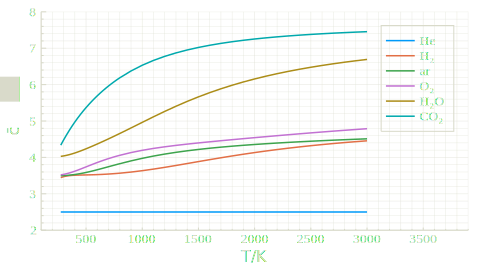
\includegraphics[width=12.0cm]{fig/A0304-pt-CP-Edited.pdf}
        \end{figure}
    \end{frame}
    %-------------------------------------------------------------------------------------------

    % !j 96 -i8
    %-------------------------------------------------------------------------------------------
    \begin{frame}{Substância Incompressível --- com $dv = 0$}\vspace*{-2em}
        \begin{columns}
        \column{0.55\textwidth}
            \begin{itemize}
                \item<1-> Comportamento \emph{aproximado} por \alert{sólidos} e \alert{líquidos};
                \item<2-> Processos a \alert{$P$-const.} idênticos aos a \alert{$v$-const.};
                \item<3-> Portanto: \alert{$c_P  =  c_v  =  c$}  o  \alert{calor  específico  de
                    substância incompressível};
                \item<4->    Tem-se    \alert{$c\!:\!c(T)$},     \alert{$u\!:\!u(T)$},     porém
                    \alert{$h\!:\!h(T, P)$}.
            \end{itemize}
            \begin{align}
                \uncover<5->{%
                    \alert{\Delta u} & = u_2 - u_1 \alert{= \int_1^2 c(T)\,dT},\nonumber\\}
                \uncover<6->{%
                    \alert{\Delta h} & \alert{= \Delta u + v\Delta P}.\nonumber}
            \end{align}
        \column{0.45\textwidth}
            \begin{figure}
                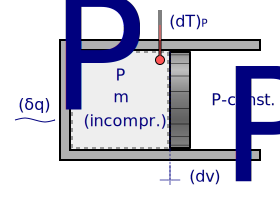
\includegraphics[width=5.0cm]{fig/A0304-pt-IncompHeating.pdf}
            \end{figure}
        \end{columns}
    \end{frame}
    %-------------------------------------------------------------------------------------------

%-----------------------------------------------------------------------------------------------
\section{Tópicos de Leitura}
%-----------------------------------------------------------------------------------------------

    %------------------------------------------------------------------------------------------
    \begin{frame}[allowframebreaks]{Tópicos de Leitura}
        \begin{thebibliography}{Çengel, Y.~A., 2013}
            \bibitem[Çengel, Y.~A., 2013]{2013-CengelYA+BolesMA-AMGH}
                Çengel, Y.~A. e Boles, M.~A.
                \newblock{%
                    {\em Termodinâmica $7^\mathrm{a}\!$ Edição\/}.
                    \alert{Seções~4-3 a 4-5.}
                }
                \newblock{\footnotesize AMGH. Porto Alegre. ISBN 978-85-8055-200-3.}
        \end{thebibliography}
    \end{frame}
    %------------------------------------------------------------------------------------------

    % Finishes with stunning image, with credit
    \ArtEndW{horizon-768759_1280}{jpg}{txt}

%-----------------------------------------------------------------------------------------------
\end{document}
%-----------------------------------------------------------------------------------------------

